\documentclass[xcolor=table]{beamer}

\usepackage{graphicx}
\usepackage{wrapfig}
\usepackage{url}

\title{GV120 - Politics and Economics Policies}
\subtitle{University of Essex - Department of Government}
\date{Week 2 -- 11 October, 2019}				% or you can specify a date, just write it down instead of "\today"
\author{Lorenzo Crippa} 

\usetheme[progressbar=frametitle]{metropolis}
\usecolortheme{seahorse}						% try others: wolverine; crane...

\begin{document}
\frame{
\titlepage
}

\frame{
\frametitle{Your GTA}

\begin{center}
Hi! My name is Lorenzo Crippa,

Email: l.crippa@essex.ac.uk

Office: 5B.153 (Department of Government)

Office hour: Wednesday 15:00 to 16:00
\end{center}
}

\frame{
\frametitle{Basic housekeeping rules}
\begin{itemize}
\item Class on Friday, 14:00 to 15:00
\item Room 3.105
\item A more participated class
\item Sharing handouts: send them to me and I forward them to the class?
\item Presentations but also Q\&A about any topic related to the module

\end{itemize}
}

\frame{
\frametitle{Bottom-up organisation}
\begin{center}
Let's introduce ourselves to each other!
\end{center}

\begin{itemize}
\item Your name
\item What do you study?
\item Why have you chosen this degree?
\end{itemize}
}

\frame{
\frametitle{Class organisation}
\begin{itemize}
\item Form groups (best if they are groups of 2)
\item Choose a topic and a related reading
\item Sign up your names on the table that is circulating
\end{itemize}

\begin{center}
\url{https://www.randomlists.com/team-generator}
\end{center}
}



\frame{
\frametitle{Rough timetable}

\begin{table}[]
\centering
%\resizebox{\textwidth}{!}{%
\begin{tabular}{|c|l|}
\hline
{\color[HTML]{333333} \textbf{Week number}} & \multicolumn{1}{c|}{{\color[HTML]{333333} \textbf{What are we going to do?}}}                                        \\ \hline
{\color[HTML]{333333} 2}                    & {\color[HTML]{333333} -- organisation and introduction}                                                              \\ \hline
{\color[HTML]{333333} 3}                    & {\color[HTML]{333333} -- 1 group presents}                                                                           \\ \hline
{\color[HTML]{333333} 4}                    & {\color[HTML]{333333} -- 2 groups present}                                                                           \\ \hline
{\color[HTML]{333333} 5}                    & {\color[HTML]{333333} -- 2 groups present}                                                                           \\ \hline
{\color[HTML]{333333} 6}                    & {\color[HTML]{333333} \begin{tabular}[c]{@{}l@{}}-- discuss take-home assignment\\ -- 1 group presents?\end{tabular}} \\ \hline
{\color[HTML]{333333} 7}                    & {\color[HTML]{333333} \begin{tabular}[c]{@{}l@{}}-- discuss in-lecture test\\ -- 1 group presents?\end{tabular}}      \\ \hline
{\color[HTML]{333333} 8}                    & {\color[HTML]{333333} EXTRA SLOT: catch up with presentations?}                                                      \\ \hline
{\color[HTML]{333333} 9}                    & {\color[HTML]{333333} -- 2 groups present}                                                                           \\ \hline
{\color[HTML]{333333} 10}                   & {\color[HTML]{333333} -- 1 group presents}                                                                           \\ \hline
{\color[HTML]{333333} 11}                   & {\color[HTML]{333333} EXTRA SLOT: catch up with presentations?}                                                      \\ \hline
\end{tabular}%
%}
\end{table}

}

\frame{
\frametitle{What makes for a good presentation? (I part)}
\begin{center}
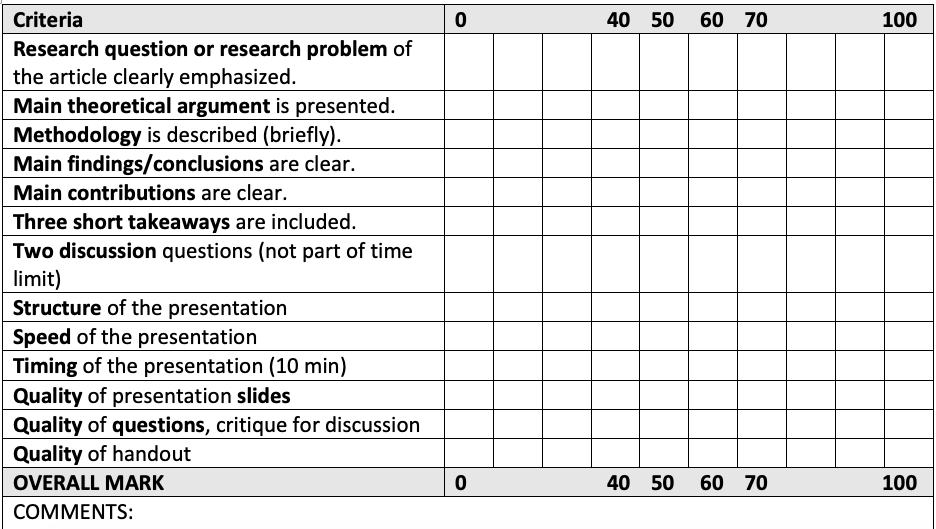
\includegraphics[height=6cm]{evaluation}
\end{center}
}

\frame{
\frametitle{What makes for a good presentation? (II part)}
\begin{enumerate}
\item Understanding the paper
	\begin{enumerate}
	\item Research context
	\item Main research question
	\item Main argument
	\item Methodology
	\item Main findings and contributions
	\end{enumerate}
\item Beyond the paper
	\begin{enumerate}
	\item Critical points (2 questions, issues, comments, critiques)
	\item Stimulate a discussion with the audience
	\end{enumerate}
\item Speed and style
	\begin{enumerate}
	\item 10 minutes per group to present 
	\item A clear and complete presentation
	\end{enumerate}
\end{enumerate}
}

\frame{
\frametitle{Example of a presentation by me}
Kaczmarek, S. and A. L. Newman (2011). ``The Long Arm of the Law: Extraterritoriality and the National Implementation of Foreign Bribery Legislation''. \emph{International Organization}, 65 (4): 745-770.

(Handout will be sent to the mailing list of the class this afternoon)

}

\frame{
\frametitle{1. Research context}
\begin{itemize}
\item {\bf Context}: Foreign bribery is nowadays a criminal offence (1997 OECD Anti-Bribery Convention)
\item U.S. anti-bribery law applies also to non-American citizens
\item {\bf Problem}: Regulating foreign bribery requires collective action by sovereign states. 
\item Clash between individual and societal interests
\end{itemize}
}

\frame{
\frametitle{2. Research question and argument}
\begin{itemize}
\item {\bf Res. Question}: What is the reaction of sovereign states to the extraterritorial application of U.S. anti-bribery law?
\item Theory supports competing answers: Spill-over (+) or competition (--)?
\item {\bf Authors' argument}: U.S. behaviour has a positive impact on states' application of their own anti-bribery laws
\end{itemize}
}

\frame{
\frametitle{3. Methodology and findings}
\begin{itemize}
\item {\bf Data}: Actual instances of prosecution for foreign bribery 
\item {\bf Methodology}: Discrete event-history analysis
	\begin{itemize}
	\item[--] Dependent variable: first application of anti-bribery law by a country
	\item[--] (Main) independent variable: application of U.S. anti-bribery law against a citizen of that country
	\end{itemize}
\item {\bf Findings}: Application of the U.S. anti-bribery law \emph{on average} stimulate other countries to start applying their laws
\end{itemize}
}

\frame{
\frametitle{4. Critical points and gaps}
\begin{itemize}
\item {\bf Theoretical}: By what causal link is this positive effect channelled? 
\item {\bf Methodological}: The variable for state \emph{compliance} with the OECD Convention is ordinal. What happens \emph{after} the state has first-applied its anti-bribery laws?
\end{itemize}
}

\frame{
\frametitle{Conclusion}
\begin{center}
Questions? Doubts? 

Don't hesitate to ask me or simply drop me an email.

See you next week!
\end{center}
}

\end{document}
